\section{Experimental Details}

In this section, we provide detailed descriptions of the datasets and evaluation metrics used across all benchmarks in this paper.




\subsection{Semantic Segmentation: Linear Probing}
\label{app:exp-details:segmentation-probing}

\paragraph{Datasets and Metrics} 
We evaluate semantic segmentation performance of DINOv3 obtained via linear probing on three benchmark datasets: ADE20k~\citep{zhou2017scene}, VOC12~\citep{pascal-voc-2012}, and Cityscapes~\citep{cordts2016cityscapes}. The evaluation metric reported is the standard mean Intersection-over-Union (mIoU).

\paragraph{Evaluation Protocol} 
To assess the quality of the dense features, we train a linear classifier on the training set of each benchmark. This linear layer is applied on top of the patch output features (after layer normalization) of the frozen backbone, with the features further normalized using a trained batch normalization layer. For all backbones, we perform a hyperparameter sweep using the AdamW optimizer, varying the learning rate over \(\{1 \times 10^{-4}, 3 \times 10^{-4}, 1 \times 10^{-3}\}\) and weight decay over \(\{1 \times 10^{-4}, 1 \times 10^{-3}\}\).

\subsection{Depth Estimation: Linear Probing}
\label{app:exp-details:depth-probing}

\paragraph{Datasets and Metrics} 
We evaluate the quality of DINOv3 features for geometric tasks on the depth benchmarks NYUv2~\citep{silberman2012indoor} and KITTI~\citep{geiger2013vision} datasets. 
Results are reported using the Root Mean Squared Error (RMSE) metric.

\paragraph{Evaluation Protocol}
To assess the quality of the dense features, we train a linear classifier on the training set of each benchmark. This linear layer is applied on top of the patch output features (after layer normalization) of the frozen backbone, with the features further normalized using a trained batch normalization layer.
For all backbones, we perform a hyperparameter sweep using the AdamW optimizer, varying the learning rate over \([1 \times 10^{-4}, 3 \times 10^{-4}, 1 \times 10^{-3}]\) and weight decay over \([1 \times 10^{-4}, 1 \times 10^{-3}]\).

\subsection{3D Keypoint Matching}
\label{app:exp-details:keypoint-matching}

\paragraph{Datasets and Metrics}
Geometric correspondence is evaluated on the NAVI dataset~\citep{jampani2023navi}, and semantic correspondence on the SPair dataset~\citep{min2019spair71k}.
For NAVI, we use images resized to a side length of 448/512 pixels  for models with patch size 14/16.
For SPAir, we use images resized to a side length of 896/1024 pixels for models with patch size 14/16.
To measure performance, we report the correspondence recall, \ie the percentage of correspondences falling into a specified distance.

\paragraph{Evaluation Protocol}
For NAVI, we follow the protocol defined in Probe3D~\citep{banani2024probing}.
Specifically, we subsample 1/4 of the object views, and for each source view select another dest.~view within a maximum rotation of 120 degrees to create an image pair (source, dest.) to perform patch matching on. 
For each image pair, each patch of source (within the object) is matched to a patch in dest. 
The top-1000 matches with highest cosine similarity are kept for evaluation, and a 3D distance error is computed for each match based on the known camera pose and depth maps of both images. 
This allows to compute recall errors with varying thresholds, for which we use thresholds of 1cm, 2cm, and 5cm.
We then compute the average recall across thresholds as the correspondence recall.

For each evaluated backbone, we use the features of the final layer, and evaluate them with and without the final layer norm applied. 
This is because we noticed bad performance for some models when applying the final layer norm.
We report the maximum of both results.

\subsection{Unsupervised Object Discovery}
\label{app:exp-details:object-discovery}

\paragraph{Datasets and Metrics}
For this task, the objective is to generate a single bounding box per image that highlights any object depicted in the scene. We follow the protocol of \citet{simeoni2021localizing} for unsupervised object discovery and evaluate all backbones on the detection benchmarks VOC07~\citep{pascal-voc-2007}, VOC12~\citep{pascal-voc-2012}, and COCO20K~\citep{Lin2014cocodataset,Vo20rOSD}. COCO20K is a subset of the COCO2014 trainval dataset~\citep{Lin2014cocodataset}, consisting of 19,817 randomly selected images, as proposed in \citep{Vo20rOSD} and commonly used for this task. For each image, a single bounding box is generated. For evaluation, we use the \textit{Correct Localization} (CorLoc) metric, which computes the percentage of correctly localized boxes. A predicted box is considered correct if its \textit{intersection over union} (IoU) with any ground-truth bounding box exceeds 0.5.

\paragraph{Evaluation Protocol}
To evaluate the quality of the image encoders, we employ the TokenCut strategy~\citep{wang2023tokencut}. This method organizes image patches into a fully connected graph, where the edges represent similarity scores between pairs of patches, computed using backbone features learned by the transformer. The salient object patches are identified by applying the Normalized Cut algorithm, which solves a graph-cut problem. A bounding box is then fitted to the resulting salient object mask.
All images are input to the encoders at their full resolution, and we use the patch output features for all image encoder. To account for differences in feature distributions among models, we perform a sweep over TokenCut’s unique hyperparameter: the similarity threshold used in graph construction. Specifically, we vary the threshold between 0 and 0.4 in increments of 0.05.

\subsection{Video Segmentation Tracking}
\label{app:exp-details:tracking}

\paragraph{Datasets and Metrics}
For this task, we use the DAVIS~2017 \citep{pont20172017}, YouTube-VOS \citep{xu2018youtubevos} and MOSE~\citep{ding2023mose} datasets.
DAVIS defines a training set of 60 videos and a validation set of 30 videos for which all frames are annotated with ground-truth instance segmentation masks.
For YouTube-VOS, only the training set is annotated and publicly available, while the validation set is gated behind an evaluation server.
To mimic the DAVIS setup, we take a random subset of 2758 annotated videos (80\%) as the training set and the remaining 690 videos (20\%) as the validation set.
In a similar fashion, we split the MOSE dataset into 1206 videos for validation and 301 for testing.
For all datasets, we evaluate performance using the standard \(\JnF\)-mean metric \citep{perazzi2016benchmark}, which combines the region similarity (\(\mathcal{J}\)) and contour accuracy (\(\mathcal{F}\)) scores.
Only the objects annotated in the first frame are tracked and evaluated, while objects that appear later in the video are ignored, even if their ground-truth masks are annotated.

\paragraph{Evaluation Protocol}
Similar to \citet{rajasegaran2025empirical}, we implement a non-parametric protocol for label propagation based on patch similarity, which is computed as a cosine similarity between features extracted from a frozen DINOv3 backbone.
We assume that the first frame of the video is labeled with instance segmentation masks, which we represent as a one-hot vector per patch.
For each frame, we compute the cosine similarity between all its patch features, all patches of the first frame, and all patches of a small number of past frames.
Focusing on a single patch in the current frame, we consider the \(k\) most similar patches within a spatial neighborhood, and compute a weighted average of their labels to obtain a prediction for the current patch.
After processing one frame, we move to the next one, treating the previous predictions as soft instance segmentation labels.
When forwarding individual frames through the backbone, we resize the image such that the shortest side matches a certain size, preserving aspect ratio up to the nearest multiple of the patch size.\footnote{
For example, DAVIS videos are natively \(480{\times}854\) and we want to process them at resolution 960.
For a model with patch size 16, we resize the frames to \(960{\times}1712\) with a slight horizontal stretch, resulting in a \(60{\times}107\) feature map.
Instead, for a model with patch size 14, we resize the frames to \(966{\times}1708\) with a slight vertical stretch, resulting in a \(69{\times}122\) feature map.
}
Patch similarity and label propagation are computed at the resolution of the resulting features, then the mask probabilities are bilinearly resized to the native resolution for computing \(\JnF\).
We consider several hyperparameter combinations, \eg the number of past frames to use as context, the number of neighbors \(k\), and the size of the spatial neighborhood, as summarized in \cref{tab:exp-details-tracking-hyperparameters}.
We perform hyperparameter selection on the training set of DAVIS, and then apply the best combination to the test splits of all datasets.

\begin{table}[tb]
    \centering
    \caption{
        List of hyperparameters evaluated for video segmentation tracking on the training split of DAVIS 2017 \citep{pont20172017}.
        The best hyperparameters, highlighted, are applied to all datasets.
    }
    \label{tab:exp-details-tracking-hyperparameters}
    \begin{tabular}{@{}ccccc@{}}
        \toprule
        Max context length & Neighborhood mask size & Neighborhood mask shape & Top-K & Temperature \\
        \midrule
        \phantom{0}7 & 12 & Square & \phantom{0}5 & 0.2\phantom{0} \\
        \phantom{0}7 & 12 & Circle & \phantom{0}5 & 0.2\phantom{0} \\
        \phantom{0}7 & \phantom{0}5 & Square & \phantom{0}5 & 0.2\phantom{0} \\
        \phantom{0}7 & 24 & Square & \phantom{0}5 & 0.2\phantom{0} \\
        \rowcolor{lightgray} \phantom{0}7 & \(\infty\) & --- & \phantom{0}5 & 0.2\phantom{0} \\
        \phantom{0}7 & 12 & Square & \phantom{0}5 & 0.01  \\
        \phantom{0}7 & 12 & Square & \phantom{0}5 & 0.1\phantom{0}  \\
        \phantom{0}7 & 12 & Square & \phantom{0}5 & 0.7\phantom{0}  \\
        \phantom{0}4 & 12 & Square & \phantom{0}5 & 0.2\phantom{0}  \\
        10 & 12 & Square & \phantom{0}5 & 0.2\phantom{0}  \\
        15 & 12 & Square & \phantom{0}5 & 0.2\phantom{0}  \\
        \phantom{0}7 & 12 & Square & \phantom{0}3 & 0.2\phantom{0}  \\
        \phantom{0}7 & 12 & Square & 10 & 0.2\phantom{0}  \\
        \phantom{0}7 & 12 & Square & 15 & 0.2\phantom{0}  \\
        15 & 12 & Circle & 10 & 0.1\phantom{0} \\
        15 & 24 & Circle & 10 & 0.1\phantom{0} \\
        15 & 36 & Circle & 10 & 0.1\phantom{0} \\
        15 & \(\infty\) & --- & 10 & 0.1\phantom{0} \\
        \bottomrule
    \end{tabular}
\end{table}

\subsection{Video Classification}
\label{app:exp-details:video-classification}

\paragraph{Datasets and Metrics}
We evaluate DINOv3 on video classification using the UCF101 \citep{soomro2012ucf101}, Something-Something V2 \citep{goyal2017something}, and Kinetics-400 \citep{kay2017kinetics} datasets.
At a high level, we extract a fixed number of frames from each video, encode them with a frozen backbone, collect all patch features into a flat sequence, which we then feed to a shallow transformer-based classifier trained with regular supervision on a set of labeled videos.
In previous work, \eg \citep{assran2025vjepa2}, this protocol is referred to as an \emph{attentive probe}, a hint to the \emph{linear probes} used for image classification.
In the following paragraphs, we describe our implementation of the protocol.

\paragraph{Training}
At training time, we select 16 frames at random temporal locations from each video, keeping track of the corresponding timestamps.
We also sample the parameters of a spatial crop that covers between 40\% and 100\% of the area--these parameters will be shared across all frames of the video to avoid jittering.
We then process each frame with DINOv3 as an independent \(256{\times}256\) image, extracting \(16{\times}16\) patch features and discarding the CLS token.
For each patch, we keep track of its spatial coordinates defined on a \([0,1]^2\) box.
The patch features from all frames are linearly projected to \(1024\) dimensions, concatenated into a flat sequence of length \(16{\times}16{\times}16=4096\), and then fed to four self-attention blocks that model the spatial and temporal relationships between the patches.
To ensure the model has access to positional information, we inject the timestamp and spatial coordinates of each patch both as an additive sin-cos embedding before the blocks \citep{vaswani2017attention}, and as a 3D factorized RoPE with random spatial rotations in each attention head~\citep{heo2024rotary}.
After the four blocks, we apply a cross-attention block with a single position-less learnable query to aggregate the information from all patches into a single vector, which is then linearly projected to obtain the final classification logits.
The stack of self-attention blocks, the cross-attention block, the positional embeddings, and the final projection constitute the video classifier, which we train for 20 epochs with batch size 64 with a standard cross-entropy loss.
In practice, we train a set of classifiers in parallel, one for each combination of learning rate
\(\{1\cdot 10^{-4}, 2\cdot 10^{-4}, 5\cdot 10^{-4}, 1\cdot 10^{-3}, 2\cdot 10^{-3}, 5\cdot 10^{-3}\}\)
and weight decay
\(\{10^{-3}, 10^{-2}, 10^{-1}\}\).
For each dataset, we use 90\% of the training set to update the model parameters, 10\% of the training set to choose the best combination of learning rate and weight decay, and finally report performance of the chosen model on the validation split.

\paragraph{Inference}
At inference time, we follow a deterministic strategy to sample a single clip per video: we take the first frame, the last frame, and uniformly-spaced frames in between, for a total of 16.
From each frame, we crop the largest center square and resize it to \(256{\times}256\) pixels, possibly losing information from the sides of rectangular videos.
We then feed these frames to DINOv3 and to the classifier to obtain a prediction for the video.
Alternatively, we follow \citet{assran2025vjepa2} and perform test-time augmentation (TTA) by selecting multiple frame sequences and multiple spatial crops, processing them independently and then averaging the class probabilities to obtain the final prediction.
Clip sampling is exemplified in \cref{fig:video_attn_pool_clip_sampling}.

\paragraph{Baselines}
For the chosen baseline models, we use the same evaluation protocol, \ie feature extraction, classifier architecture, training procedure and inference protocol, with a few differences.
The input resolution is \(256{\times}256\) pixels for models that use patch size 16, and \(224{\times}224\) pixels for patch size 14.
This way, all backbones yield an identical number of tokens, and therefore afford the same amount of computation in the classifier.
All models process videos frame by frame independently, since they are trained on images.
The only exception is V-JEPA 2, to which we feed whole clips to extract time-aware features.
Since V-JEPA 2 reduces the temporal axis by a factor of two, \eg yielding 8 time steps given 16 frames as input, we duplicate each patch token to match the sequence length of other models.

\begin{figure}[t]
    \centering
    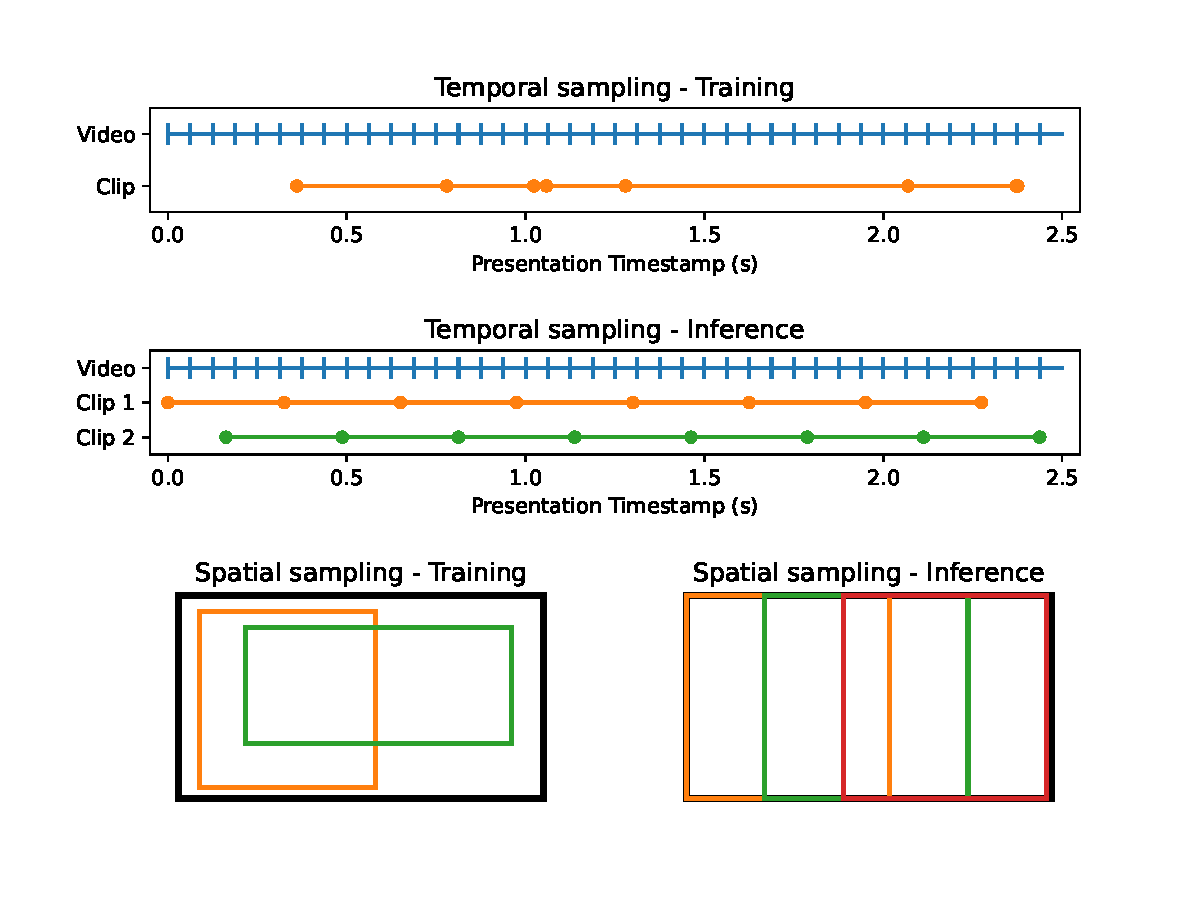
\includegraphics[width=\linewidth]{figures/evals/video_attention_pooling_clip_sampling.pdf}
    \caption{
        Sampling clips for video classification.
        Choosing a clip for training or inference means determining the coordinates of a spatial crop and which frames/timestamps to sample.
        At training time, we sample clips at random by choosing random frames from the whole video and by applying a spatial crop that covers \(\ge40\%\) of the area.
        At inference time, we select clips in a deterministic way.
        Spatially, we take the three largest square crops aligned to the left, middle and right.
        Temporally, we take two overlapping sets of frames such that they cover as much of the video as possible and their timestamps interleave.
    }
    \label{fig:video_attn_pool_clip_sampling}
\end{figure}



\subsection{Image Classification with Linear Probing}
\label{app:exp-details:classification}

\paragraph{Datasets and Metrics}
We evaluate the global quality of the DINOv3 model using the widely adopted linear probing evaluation. 
We train a linear transform on the training set of ImageNet-1k~\citep{deng2009imagenet} and evaluate results on the val set.
We assess the generalization quality of the model by evaluating the transfer to classification test sets: ImageNet-\textbf{V2}~\citep{recht2019imagenet} and \textbf{ReaL}~\citep{beyer2020imagenetreal}, which provide alternative sets of images and labels for ImageNet, designed to test for overfitting on the original ImageNet validation set. Additionally, we consider the \textbf{R}endition~\citep{hendrycks2021many} and \textbf{S}ketch~\citep{wang2019learning} datasets, which present stylized and artificial versions of ImageNet classes; the \textbf{A}dversarial~\citep{hendrycks2021natural} and \textbf{Obj}ectNet~\citep{barbu2019objectnet} datasets, which contain deliberately challenging examples; and the \textbf{C}orruptions~\citep{hendrycks2019benchmarking} dataset, which measures robustness to common image corruptions. 
We report top-1 classification accuracy as the evaluation metric for all datasets but ImageNet-C, for which we report the mean corruption error (mCE, see \citep{hendrycks2019benchmarking}).

For fine-grained datasets, we consider the same collection of 12 datasets from \citet{oquab2024dinov2}, which we call Fine-S here: Food-101~\citep{dataset-food101}, CIFAR-10~\citep{krizhevsky2009learning}, CIFAR-100~\citep{krizhevsky2009learning}, SUN397~\citep{dataset-sun397}, StanfordCars~\citep{dataset-stanfordcars}, FGVC-Aircraft~\citep{dataset-aircraft}, VOC 2007~\citep{pascal-voc-2007}, DTD~\citep{dataset-dtd}, Oxford Pets~\citep{dataset-pets}, Caltech101~\citep{dataset-caltech101}, Flowers~\citep{dataset-flowers}, and CUB200~\citep{dataset-cub}, as well as the larger datasets Places205~\citep{zhou2014learning}, iNaturalist 2018~\citep{van2018inaturalist}, and iNaturalist 2021~\citep{van2021benchmarking}.

\paragraph{Evaluation Protocol}
For the larger datasets ImageNet, Places205, iNaturalist 2018 and iNaturalist 2021, we use the following procedure.
For each baseline, we train a linear layer on the final features of the CLS token (after the layer norm) using the ImageNet-1k training set~\citep{deng2009imagenet}. 
Specifically, we use SGD with a momentum of 0.9, and train for 10 epochs with a batch size of 1024.
We sweep the learning rates $\{1 \times 10^{-4}, 2 \times 10^{-4}, 5 \times 10^{-4}, 1 \times 10^{-3}, 2 \times 10^{-3}, 5 \times 10^{-3}, 1 \times 10^{-2}, 2 \times 10^{-2}, 5 \times 10^{-2}, 1 \times 10^{-1}, 2 \times 10^{-1}, 5 \times 10^{-1}, 1 \times 10^{0}, 2 \times 10^{0}, 5 \times 10^{0}\}$ and weight decay values $\{0, 1e-5\}$ and use the validation set of ImageNet-1k to select the best combination.
During training, we use random resize crop augmentation with standard Inception-crop parameters.
For the datasets in Fine-S, following \citet{oquab2024dinov2}, we use a lighter weight evaluation using scitkit-learn's  LogisticRegression implementation with the L-BFGS solver.

In both cases, we evaluate models at resolutions resulting in 1024 patch tokens, that is, $448 \times 448$ for patch size 14, and $512 \times 512$ for patch size 16.
The images are resized such that the shorter side matches the chosen side length, then take the central square crop.

\subsection{Instance Recognition}
\label{app:exp-details:recognition}

\paragraph{Datasets and Metrics}
We use the Oxford and Paris datasets for landmark recognition~\citep{radenovic2018revisiting}, the Met dataset featuring artworks from the Metropolitan Museum~\citep{ypsilantis2021met}, and AmsterTime, which consists of modern street view images matched to historical archival images of Amsterdam~\citep{yildiz2022amstertime}.
In \cref{tab:results-instance-recognition}, we report mean average precision (mAP) for Oxford-Hard, Paris-Hard, and AmsterTime, and global average precision (GAP) for Met.
In \cref{app:tab:results-instance-retrieval}, we additional give mAP for Oxford-Medium and Paris-Medium, as well as the additional metrics GAP- and accuracy (see \citep{ypsilantis2021met}).
For Oxford and Paris, we resize all images such that the larger side is 224 pixels long, keeping the aspect ratio, then take a full center crop, yielding an image of resolution of $224 \times 224$.
For AmsterTime, we resize all images such that the shorter side is 256 pixels long, keeping the aspect ratio, then take a center crop of size $224 \times 224$.
For Met, we evaluate all images close to their original resolution, resizing both to the nearest multiple of patch size (resulting in a long side 508/512 for patch size 14/16).

\paragraph{Evaluation Protocol}
The image similarity is computed using cosine distance between the CLS tokens computed for query and target images.
We follow the evaluation protocols of \citep{radenovic2018revisiting} for Oxford and Paris, of \citep{yildiz2022amstertime} for AmsterTime, and of \citet{ypsilantis2021met} for Met.
For Met, this includes tuning the hyperparameters k and $\tau$ with a grid search, optimizing GAP on the validation set of Met, and whitening the features using a PCA estimated on the training set of Met.


\subsection{Object Detection}
\label{app:exp-details:detection}

\paragraph{Datasets and Metrics}
We evaluate DINOv3 on object detection on the COCO \citep{Lin2014cocodataset} and COCO-O \citep{mao2023cocoo} datasets.
COCO is a standard benchmark for object detection, covering 80 object categories, and containing 118k training images and 5k validation images.
COCO-O is an evaluation-only dataset with the same categories as COCO, but in more challenging visual conditions, such as scenes with significant occlusions, cluttered backgrounds, and varying lighting conditions.
For training the object detection model, we also leverage the Objects365 \citep{shao2019objects365} dataset, which contains 2.5M images and covers 365 object categories, a subset of which maps directly to COCO classes.
For both COCO and COCO-O, we report mean Average Precision (mAP) computed at IoU thresholds of \([0.5:0.05:0.95]\).

\paragraph{Architecture}
Our approach builds upon the Plain-DETR~\citep{lin2023plaindetr} implementation, with several modifications.
We do not fuse the transformer encoder into the \emph{backbone}, but keep it as a separate module, similar to the original DETR \citep{carion2020detr}.
This allows us to keep the DINOv3 backbone completely frozen during training and inference, making it the first competitive detection model to do so.
From a DINOv3 ViT-7B/16 backbone, we extract features from four intermediate layers, namely \([10, 20, 30, 40]\).
For each patch, we concatenate intermediate features channel-wise, giving a feature dimension of \(4 \cdot 4096 = 16384\), which is further increased by the windowing strategy described below.
The backbone features feed into the \emph{encoder}, which is a stack of 6 self attention blocks with embedding dimension of 768.
The \emph{decoder} is a stack of 6 cross attention blocks with the same embedding dimension, where 1500 ``one-to-one'' queries and 1500 ``one-to-many'' queries attend to the patch tokens of the encoders to predict bounding boxes and class labels.

\paragraph{Image Pre-Processing}
Training is performed in three stages as described below, one with a base image resolution of 1536 pixels and two with a base resolution of 2048.
Following DETR, we apply random horizontal flipping ($p=0.5$), followed by either
(i) random resizing, where the shortest side is uniformly sampled between 920 pixels (resp. 1228) and the base resolution of the stage (1536 or 2048), or
(ii) a random crop retaining 60--100\% of the original image area, followed by resizing as in (i).
At evaluation time, images are resized so that the shortest side is 2048 without additional augmentation, and both sides are rounded up to the nearest multiple of the patch size.

\paragraph{Windowing strategy}
We then apply a windowing strategy that combines a global view of the image with smaller views, to allow the backbone to process objects at all scales. The number of windows is fixed to $3 \times 3$, and their sizes vary according to the input resolution.
As an example, for an image of size \(1536 \times 2304\):
\begin{enumerate}
    \item
    The image is divided into \(3 \times 3\) non-overlapping windows of size \(512 \times 768\).
    Each window is forwarded through the backbone, resulting in \(32 \times 48\) patch tokens of dimension 16384.
    The features of all windows are spatially reassembled into a \((3 \cdot 32) \times (3 \cdot 48)\) feature map.
    \item
    The whole image is resized to \(512{\times}768\) and forwarded through the backbone, resulting in a feature map of \(32{\times}48\) patch tokens of dimension 16384.
    These features are then bilinearly upsampled to \(96{\times}144\), matching the size of the windowed feature map.
    \item
    Finally, the features maps from steps 1 and 2 are concatenated channel-wise, resulting in a \(96{\times}144\) feature map of dimension \(2 \cdot 16384 = 32768\).
    This feature map is then flattened as a sequence of \(96*144\) tokens and fed to the encoder.
\end{enumerate}

\paragraph{Training}

We follow a training curriculum in three stages, using the Objects365 dataset~\citep{shao2019objects365} and the COCO dataset~\citep{Lin2014cocodataset} at increasing resolutions.
Throughout training, we use the AdamW optimizer~\citep{loshchilov2017decoupled} with a weight decay of 0.05.
Following DETR, we use the Focal Loss~\citep{lin2018focallossdenseobject} as classification loss, with a weight of 2, L1 loss as bounding box loss with a weight of 1, complemented by the GIoU~\citep{rezatofighi2019generalizedintersectionunionmetric} loss with a weight of 2.
The stages are as follows:
\begin{enumerate}
    \item 
    We begin training on Objects365 at base resolution 1536 pixels.
    We train for 22 epochs with global batch size of 32, which we distribute over 32 GPUs.
    After an initial warmup of 1000 steps, the learning rate is set to \(5\cdot10^{-5}\) and is divided by 10 after the 20th epoch.
    \item
    We then continue training on Objects365 at base resolution 2048 pixels.
    We train for for 4 epochs with learning rate \(2.5\cdot10^{-5}\).
    \item 
    We finish training by doing 12 epochs on COCO at base resolution 2048.
    After a linear warmup of 2000 iterations, the learning rate follows a cosine decay schedule, starting at \(2.5\cdot10^{-5}\) and reaching \(2.5\cdot10^{-6}\) at the 8th epoch.
    In this part we use the IA-BCE classification loss~\citep{cai2024aligndetrenhancingendtoendobject} instead of the simple Focal Loss from DETR.
    We observed this loss to increase the model performance at transfer time, but not at pretraining time.
    As this loss mixes class and box information, it brings its full potential if the box predictions are already well initialized.
    The GIoU loss weight is set to 4 in this part to encourage better box alignment.
\end{enumerate}

\paragraph{Test-Time Augmentation}
At test time, we follow the inference procedure described above, resizing images such that the short side is 1536 or 2048.
At those resolutions, the COCO mAP is 65.4 and 65.6, respectively.
Alternatively, we can apply the test-time augmentation (TTA) strategy from \citet{bolya2025perception}, which consists in flipping and resizing the image to multiple resolutions, and merging the predictions with SoftNMS~\citep{Bodla_2017_ICCV}.
Specifically, each image is processed at resolutions of \([1536, 1728, 1920, 2112, 2304, 2496, 2688, 2880]\), yielding an mAP of 66.1.

\subsection{Semantic Segmentation}
\label{app:exp-details:segmentation-system}

\paragraph{Datasets and Metrics}
We evaluate DINOv3 on semantic segmentation on the ADE20k~\citep{zhou2017scene}, Cityscapes~\citep{cordts2016cityscapes}, COCO-Stuff~\citep{caesar2018coco}, and VOC 2012 \citep{pascal-voc-2012} datasets. 
ADE20k is a widely used benchmark for semantic segmentation with 150 semantic categories, varying from outdoor scenery to images of people and objects inside a house. 
In addition, COCO-Stuff and Hypersim \citep{roberts2021hypersim} datasets are used for pre-training the model.
COCO-Stuff is a larger dataset (118k training images) than ADE20k containing 80 thing classes and 91 stuff classes, while Hypersim is a photorealistic synthetic dataset presenting indoor scenes with 40 semantic categories, with sharper and more accurate annotations. 
More than half of the Hypersim images contain 21 or more objects, making it a good candidate for helping the model learn rich information of the scenes. 
The evaluation metric reported is mIoU for all datasets.

\paragraph{Architecture}
We adapt the ViT-Adapter and Mask2former configurations that other baselines use~\citep{wang2023onepeace}, with several differences.
First, to ensure that our backbone remains frozen and its activations are not altered, we remove the injector component of the ViT-Adapter. 
This makes our backbone output features to be directly used in the extractor module. 
Second, the embedding dimensions in the Mask2former decoder are scaled to 2048 instead of the default 1024 to adapt to our backbone output dimension of 4096, while other baselines' backbones usually present an output dimension of 1024 or 1536.
As inputs to the decoder, we extract features from four intermediate layers of the DINOv3 7B/16 backbone, namely layers \([10, 20, 30, 40]\).
We apply the final layer norm to the features of all layers and add a learned batch normalization.

\paragraph{Training Protocol}
For generating results on COCO-Stuff, we train the model using a cosine scheduler, with a 6k linear warmup and a maximum learning rate of 1.5e-5. 
The model is trained for 80k iterations, at resolution 1280 pixels.
As for training on the other datasets---ADE20k, Cityscapes and VOC 2012---we first pre-train the decoder on COCO-Stuff for 80k iterations, with a 6k linear warmup and a learning rate of 1.5e-5, following a cosine scheduler. 
This helps the model learn diverse semantic categories (171 categories) on a larger dataset than ADE20k. 
The model is then trained on Hypersim for 10k iterations at a learning rate of 2.5e-5 following a cosine scheduler with a 1.5k linear warmup. 
Corresponding to roughly 2 epochs, this step helps our model learn high-quality image-to-mask correspondence due to their photorealistic synthetic nature.
Finally, our model is trained on ADE20k for 20k iterations with a learning rate of 3e-5, again with a 1.5k linear warmup and a cosine schedule. 
We report our final result on the validation set. 
For Cityscapes and VOC 2012, learning rates of 1.5e-5 and 1e-5 are used respectively. 
For all training, a batch size of 16 and the AdamW optimizer is used.

\paragraph{Inference}
For single-scale evaluation, sliding inference is used for evaluating the models---the image is first resized at the training resolution (\eg a $400 \times 500$ image will be resized to $896 \times 1120$ pixels for ADE20k, since the model was trained at resolution 896). Then, a sliding window method is used with a stride (\eg stride of 596 pixels for ADE20k) on square crops (\eg $896 \times 896$ pixels) to generate a prediction for each crop, sliding through the image. 
These results are then aggregated and rescaled to the original image size to generate a final prediction.
For test-time augmentation, both ADE20k and VOC 2012 images were rescaled to ratios of [0.9, 0.95, 1.0, 1.05, 1.1] of the evaluation resolution, and each image was also flipped horizontally to generate a total of 10 predictions per sample. 
After sliding inference on each image, they were rescaled to the original image shape and averaged. 
COCO-Stuff 164K's TTA mIoU was obtained by simply using an additional horizontally flipped image per sample, and for Cityscapes, ratios of [1.0, 1.5, 2.0] of the evaluation resolution were applied.

\subsection{Monocular Depth Estimation}
\label{app:exp-details:depth-system}

\paragraph{Implementation Details}
Our approach differs from Depth Anything v2 (DAv2)~\citep{yang2024depthanythingv2} primarily in the configuration of image resolution, which is set to $768 \times 1024 pixels$, and the network architecture. 
The backbone is kept frozen throughout training, while a dropout rate of 0.05 is applied at the end of the DPT head~\citep{ranftl2021vision}. 
As input to the decoder, we extract features from four intermediate layers of the DINOv3 7B/16 backbone, namely layers \([10, 20, 30, 40]\).
We apply the final layer norm to the features of all layers and add a learned batch normalization.
The depth estimation output is discretized into 256 uniformly distributed bins covering the range from 0.001m to 100m. 
Training employs a base learning rate of 1e-3, scheduled using PolyLR with a power of 3.5 and an initial linear warmup phase lasting 12k iterations. 
To enhance robustness and generalization, we apply a suite of augmentations: Gaussian blur, Gaussian noise, AutoContrast, AutoEqualise, ColorJitter, rotation, and left-right flip.

\paragraph{Datasets and Metrics}
We train the model on the dataset of DAv2, which consists of synthetically generated images from the IRS, TartanAir, BlendedMVS, Hypersim, and VKITTI2 datasets.
We evaluate on five datasets: NYUv2~\citep{silberman2012indoor}, KITTI~\citep{geiger2013vision}, ETH3D~\citep{schoeps2017multiview}, ScanNet from \citep{ke2025marigold}, and DIODE~\citep{vasiljevic2019diode}.
We adopt the zero-shot scale-invariant depth setup, and report the standard metrics absolute relative error and $\delta_1$ (see~\citep{yang2024depthanythingv1}).

\subsection{Visual Geometry Grounded Transformer with DINOv3}
\label{app:exp-details:vggt}

\paragraph{Implementation Details}
Compared to the original VGGT~\citep{wang2025vggt}, we adopt the following changes:
(1) we use an image size of 592 instead of 518; this is to match the number of patch tokens that DINOv2 produces,
(2) adopting a smaller learning rate, specifically from 0.0002 to 0.0001, and 
(3) using a concatenation of the four intermediate layers of DINOv3 ViT-L rather than just the last layer as input to the downstream modules.
Interestingly, we found that using four intermediate layers brings a benefit for DINOv3, whereas doing the same for DINOv2 brings no additional performance gains.
We also experimented with a version closer to the original VGGT setup (image size 512, same learning rate, final layer), and already found this untuned version to improve over the original VGGT work across all tested benchmarks.










\subsection{Geospatial}
\label{app:exp-details:geospatial}
\paragraph{Evaluation details} %

In all of the evaluations, we keep the backbone frozen and only train lightweight classifiers or decoders that are specialized for the tasks.
For GEO-Bench classification, we train a linear classifier for 2400 iterations with a batch size of 32. We use SGD optimizer, cosine learning rate annealing, and select the best learning rate between $1\mathrm{e}{-5}$ and $1$. Unless otherwise specified, segmentation evaluations use a DPT decoder~\citep{ranftl2021vision}, with a learning rate selected based on performance on the validation set with a grid search of four values in $[3\mathrm{e}{-5}, 1\mathrm{e}{-4}, 3\mathrm{e}{-4}, 1\mathrm{e}{-3}]$.   

On LoveDA and iSAID datasets, we train an UPerNet decoder \citep{xiao2018unifiedperceptualparsingscene} for 80k iterations, with a batch size of 8, and a linear warm-up of 1500 iterations in line with \citep{wang2024mtpadvancingremotesensing}.
All other hyper-parameters such as crop size and weight decay are the same as in \citep{wang2024mtpadvancingremotesensing}.
Following previous work~\citep{tolan2024very,wang2022lovedaremotesensinglandcover}, we use a DPT head for canopy height prediction evaluations and train a Faster RCNN~\citep{ren2015faster} detector for 12 epochs for object detection tasks.

\paragraph{Satlidar dataset}

The Satlidar dataset consists in one Million of $512\times 512$ Maxar images and corresponding dense lidar measurements collected from different locations as described in Table \cref{tab:satlidar}.
The images were extracted from larger tiles, the numbers of tiles for each sub-dataset are specified in the table.       
\begin{table}[tb]
    \centering
    \caption{Description of the Satlidar dataset.}
    \label{tab:satlidar}
    \begin{tabular}{cccc}
    \toprule
    Subdataset & Path & Amount of tiles & Purpose \\  
    \midrule
Kalimantan &\tiny{\url{https://daac.ornl.gov/cgi-bin/dsviewer.pl?ds_id=1540}}&86&	train/val/test\\
OpenDC	& \tiny{\url{https://opendata.dc.gov/datasets/2020-lidar-classified-las/about}}&68&	train/val/test\\
Brazil	&	\tiny{\url{https://daac.ornl.gov/cgi-bin/dsviewer.pl?ds_id=1644}}&37&	train/val/test\\
Mozambique	&	\tiny{\url{https://daac.ornl.gov/cgi-bin/dsviewer.pl?ds_id=1521}}&144&	train/val/test\\
Neon		&	\tiny{\url{https://data.neonscience.org/data-products/DP3.30015.001}} &5366&train/val/test\\
CA20Graup	&	\tiny{\url{https://portal.opentopography.org/datasetMetadata?otCollectionID=OT.092021.6339.1}}&99&	train/val/test\\
CA17Duvall &	\tiny{\url{https://portal.opentopography.org/datasetMetadata?otCollectionID=OT.042020.6339.2}}&56&	train/val/test\\
Netherlands	&	\tiny{\url{https://geotiles.citg.tudelft.nl/}}&13& train/val/test\\
Sao Paulo	& \tiny{\url{https://daac.ornl.gov/CMS/guides/LiDAR\_Forest\_Inventory\_Brazil.html}} &4&	test \\
CA brande	& \tiny{\url{https://doi.org/10.5069/G9C53J18}} &1& test\\
\bottomrule
    \end{tabular}
\end{table}%
